% !TEX root = ../report.tex
\section{Plugin}
\label{sec:pattern-plugin}
Plugin pattern basically expands the capability of a particular software. Plugin
pattern also provides centralized, runtime configuration\cite{eaa}. An
illustration of plugin pattern is shown in Figure \ref{fig:plugin-pattern}.

\begin{figure}[H]
\centering
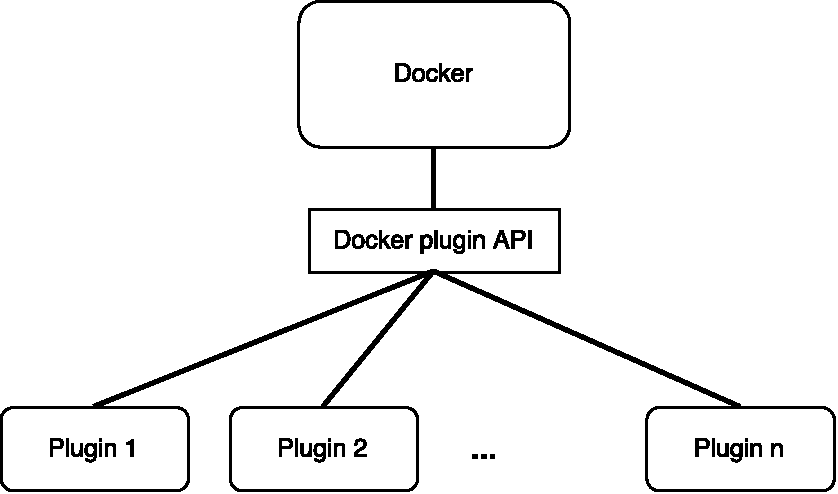
\includegraphics[scale=0.5]{5-patterns/images/plugins-pattern.pdf}
\caption{Plugin pattern illustration for Docker.}
\label{fig:plugin-pattern}
\end{figure}

\begin{patdescription}

\item [Traceability]
The existence of Docker plugin becomes apparent from its documentation, which
describes the plugin feature of Docker \cite{dockerplugindocs}.

Additionally, the directories \verb|docker/pkg/plugin/|\footnote{\url{https://github.com/docker/docker/tree/master/pkg/plugin}} and
\verb|docker/daemon/graphdriver/plugin.go|\footnote{
\url{https://github.com/docker/docker/blob/master/daemon/graphdriver/plugin.go}}
(among others) in the project's repository contain the code for discovering
plugin and the interfaces the plugin should implement.

\item [Source]
Patterns of Enterprise Application Architecture, P. 499 \cite{eaa}

\item [Issue]
%TODO joris: make neat sentence
Several of Docker users desired functionalities are not natively provided by
docker. Docker provides the mechanism so that third party custom-built tools
that provide this missing functionality to extend Docker. These customizations
mean that third party developers are able to write tools, extending Docker's
core functionality\cite{dockerpluginblog}. The additional functionality that is
added, is only usable during run time.
%TODO joris: add consequences of this issue (regarding key d's?).


\item [Assumptions/Constraints]
\begin{mynesteditemlist}
\item plugin can only extend the functionality of the Docker components if
necessary APIs are provided for certain need or use.
\end{mynesteditemlist}

\item [Solution]
Docker implements the plugin pattern to link several Docker's extendable
component's interfaces with third-party code at runtime.

\item [Rationale]  % https://docs.docker.com/engine/extend/plugin_api/
By using plugin pattern, any feature that is currently not supported natively
by Docker can be added. The users can also develop a custom code that will
exploit Docker APIs to fulfill their need.

\item [Implications]
The use of the plugin pattern means that the adaptability increases, because
plugin allow the application to be adapted with new features. For the security
concern, it means that there is extra communication over the API which has to be
secured. The security of the plugin themselves cannot be guaranteed by Docker.

\item [Related Patterns]
\begin{mynesteditemlist}
\item Broker
\end{mynesteditemlist}
\end{patdescription}

